\documentclass{standalone}

\usepackage[dvipsnames]{xcolor}
\usepackage{tikz}
\usepackage{enumitem}
\usepackage{fontspec}
\setmainfont{Roboto}
\small
\raggedright

\begin{document}
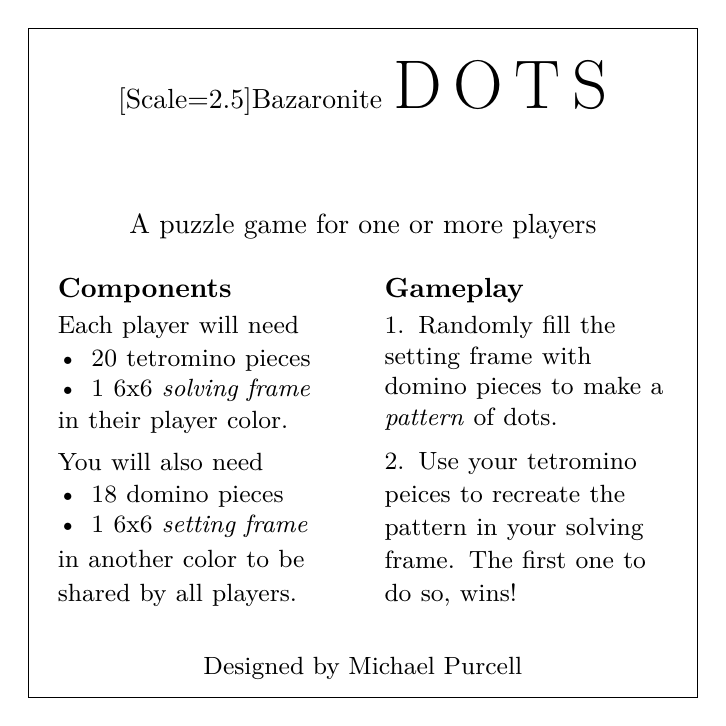
\begin{tikzpicture}
%\node[inner sep=0pt] at (0,0) {\includegraphics[width=90mm]{light_wood_background.jpg}};
%\path[draw] (-42.5mm, -42.5mm) -- (42.5mm, 42.5mm);
\node[draw, minimum width=85mm, minimum height=85mm, inner sep=0pt] at (0,0) {};
\node[anchor=north, inner sep=0pt] at (0,38.5mm) {\setmainfont[Scale=2.5]{Bazaronite}\Huge \,D\,O\,T\,S};
\node[anchor=south, text width=77.5mm, align=center, rounded corners=1mm, fill=white, opacity=0.0, text opacity=1.0] at (0,14.5mm) {A puzzle game for one or more players};


\node[fill=white, opacity=0.0, text opacity=1.0, text width=36mm, rounded corners=1mm, anchor=north, text depth=39.5mm] at (-20.75mm, 12mm) {\normalsize\textbf{Components}\\[0.5ex]\small
Each player will need
\begin{itemize}[leftmargin=*, noitemsep, topsep=0.175ex]
\item 20 tetromino pieces
%\item 2 monomino pieces
\item 1 6x6 \emph{solving frame}
\end{itemize}
in their player color.\\[1.0ex]
You will also need
\begin{itemize}[leftmargin=*, noitemsep, topsep=0.175ex]
\item 18 domino pieces
\item 1 6x6 \emph{setting frame}
\end{itemize}
in another color to be shared by all players.
};

%\node[fill=white, opacity=0.5, text opacity=1.0, text width=35mm, rounded corners=1mm, anchor=north] at (-21.25mm, -10mm) {\normalsize\textbf{Set Up}\\[1ex]\small
%\begin{itemize}[leftmargin=*, nosep]
%%\item Choose a frame.
%\item Fill one frame with randomly oriented domino pieces.
%\end{itemize}
%};
%


\node[fill=white, opacity=0.0, text opacity=1.0, text width=36mm, rounded corners=1mm, anchor=north, text depth=39.5mm] at (20.75mm, 12mm) {\normalsize\textbf{Gameplay}\\[0.5ex]\small
1. Randomly fill the\\setting~frame with domino pieces to make a \emph{pattern} of dots.
\\[1ex]
2. Use your tetromino peices to recreate the pattern in your solving frame. The first one to do so, wins!
};

\node[anchor=south, fill=white, opacity=0.0, text opacity=1.0, rounded corners=1mm] at (0,-41.5mm) {\small Designed by Michael Purcell};
\end{tikzpicture}
\end{document}